\textbf{Входные параметры:} 
 
x --- входная переменная;
 
X --- выборка: значения входов;
 
dY --- выборка пересчитанных значений оценок производной через функцию HML\_MakingVectorForNonparametricEstimatorOfDerivative3;
 
VHML\_N --- размер выборки;
 
C --- коэффициент размытости;
 
V --- тип ядра
 
 \begin{itemize}
 \item  0 --- прямоугольное (не рекомендуется);
 \item  1 --- треугольное;
 \item  2 --- параболическое (считается оптимальным);
 \item  3 --- экспоненциальное;
 \end{itemize}
 
b --- сюда возвращается 1, если все прошло хорошо и 0, если C не захватывает никаких точек выборки (тогда функция возвращает 0).

\textbf{Возвращаемое значение:}
 
 Восстановленное значение производной функции в точке.
 
\textbf{Примечание:}

В отличии от HML\_NonparametricEstimatorOfDerivative2 пересчет выборки производной производится в другой функции HML\_MakingVectorForNonparametricEstimatorOfDerivative3. Поэтому работает быстрее, но по формулам одно и тоже, что и HML\_NonparametricEstimatorOfDerivative2.

\textbf{Формула:}
\begin{eqnarray*}
\overline{dY}_j =\dfrac{\sum_{i=1}^{N}\overline{Y}_i{\Phi}'\left( \frac{\overline{X}_j-\overline{X}_i}{c}\right) \sum_{i=1}^{N}\Phi\left( \frac{\overline{X}_j-\overline{X}_i}{c}\right)-\sum_{i=1}^{N}{\Phi}'\left( \frac{\overline{X}_j-\overline{X}_i}{c}\right) \sum_{i=1}^{N}\overline{Y}_i\Phi\left( \frac{\overline{X}_j-\overline{X}_i}{c}\right)}{c\left( \sum_{i=1}^{N}\Phi\left( \frac{\overline{X}_j-\overline{X}_i}{c}\right)\right)^2 }, j=\overline{1,N}.
\end{eqnarray*}
\begin{eqnarray*}
{f}'\left( x, \overline{X},\overline{dY}, c\right) =\dfrac{\sum_{i=1}^{N}\overline{dY}_i\Phi\left( \frac{x-\overline{X}_i}{c}\right) }{\sum_{i=1}^{N}\Phi\left( \frac{x-\overline{X}_i}{c}\right) }.
\end{eqnarray*}

 \begin{figure} [h] 
   \center
   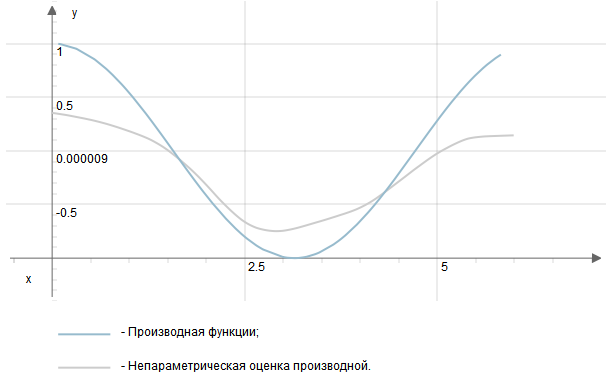
\includegraphics {HML_NonparametricEstimatorOfDerivative3.png}
   \caption{Пример работы функции} 
   \label{img:HML_NonparametricEstimatorOfDerivative3}  
 \end{figure}